\documentclass[UTF8]{beamer}
\usepackage{ctex} % 支持中文
\usepackage{amsmath}
\usepackage{amssymb} % For symbols like \mathbb{E}, \lim, \sum
\usepackage{amsthm} % For proof environments if needed (though not strictly used here)
\usepackage{booktabs} % For better table rules

% --- Theme and Appearance ---
\usetheme{Madrid} % A popular, clean theme
% \usetheme{AnnArbor} % Another good option
% \usetheme{Singapore} % Yet another option
\usecolortheme{default} % Or try others like 'whale', 'orchid'

% Remove navigation symbols ( uncomment if you want them)
\setbeamertemplate{navigation symbols}{}

% --- Custom Colors for Beamer Blocks ---
% Using standard Beamer blocks like 'block' and 'alertblock'
% Let's redefine their colors to be distinct but match the theme style somewhat.
\setbeamercolor{block title}{bg=blue!20!white, fg=black} % Default block title color
\setbeamercolor{block body}{bg=blue!5!white, fg=black}   % Default block body color

\setbeamercolor{example title}{bg=green!20!white, fg=black} % Custom for 'example' blocks
\setbeamercolor{example body}{bg=green!5!white, fg=black}

\setbeamercolor{alertblock title}{bg=red!20!white, fg=black}   % Alert block title color
\setbeamercolor{alertblock body}{bg=red!5!white, fg=black}     % Alert block body color


% --- Define math operators for better typography ---
\DeclareMathOperator{\E}{\operatorname{E}}
\DeclareMathOperator{\Var}{\operatorname{Var}}
\DeclareMathOperator{\Prob}{\operatorname{P}}

\title{第七讲 大数定律}
\author{龚鹤扬}
\institute{中国科学技术大学统计学博士} % Using \institute is standard for affiliation, split lines with \\
\date{\today}

\begin{document}

\begin{frame}
    \titlepage
\end{frame}

\begin{frame}{目录}
    \tableofcontents
\end{frame}

\section{引言}
\begin{frame}{引言:大数定律的重要性与局限}
    \framesubtitle{并非对所有随机变量都成立的普适规律}
    \begin{itemize}
        \item 本讲主题:\alert{大数定律 (LLN)} - 重要的极限定理。
        \item 核心思想:大量重复试验中,\alert{频率} $\to$ \alert{概率};样本均值 $\to$ 总体\alert{期望}。
        \item LLN:\alert{理论概率} $\leftrightarrow$ \alert{统计推断}的桥梁;多种统计方法的基础。
        \item \alert{重要}:LLN 结论依赖特定\alert{条件} (如期望存在、方差有限)。
        \item 条件不满足?LLN可能失效。反例:\alert{柯西分布},探讨条件必要性。
    \end{itemize}
\end{frame}

\section{切比雪夫不等式}
% Shrink may be needed if content is too much
\begin{frame}[shrink=5]{7.1 切比雪夫不等式 (Chebyshev's Inequality)}
    \framesubtitle{一个重要的概率上界}
    \begin{itemize}
        \item 作用:给出随机变量偏离期望概率的\alert{上界}。
        \item 特点:不依赖具体分布,仅需\alert{期望、方差}存在且有限。
    \end{itemize}
    \pause
    \begin{block}{定理 7.1 (切比雪夫不等式)}
        设随机变量 X 具有期望 $\E(X) = \mu$ 和方差 $\Var(X) = \sigma^2$ (其中 $0 < \sigma^2 < +\infty$)。
        则对于任意正数 $\epsilon > 0$,有:
        \[ \Prob(|X - \mu| \geq \epsilon) \leq \frac{\sigma^2}{\epsilon^2} \]
        或者等价地:
        \[ \Prob(|X - \mu| < \epsilon) \geq 1 - \frac{\sigma^2}{\epsilon^2} \]
    \end{block}
    \pause
    \textbf{意义与特点:}
    \begin{itemize}
        \item \alert{普适性}:条件满足时,对任何分布成立。
        \item \alert{实用性}:分布未知时的粗略估计。
        \item \alert{局限性}:界限通常较宽松。
    \end{itemize}
\end{frame}

\section{弱大数定律 (WLLN)}
% Shrink may be needed if content is too much
\begin{frame}[shrink=5]{7.2 弱大数定律 (Weak Law of Large Numbers, WLLN)}
    \framesubtitle{样本均值的依概率收敛}
    WLLN 核心:特定条件下,样本均值 \alert{依概率收敛} 于总体期望。
    \vspace{0.3cm}

    \begin{block}{定理 7.2 (切比雪夫弱大数定律)}
        设 $X_1, X_2, \dots, X_n, \dots$ 是一列\alert{相互独立}、具有相同期望 $\E(X_i) = \mu$ 和相同\alert{有限方差} $\Var(X_i) = \sigma^2 < +\infty$ 的随机变量序列。
        令样本均值为 $\bar{X}_n = \frac{1}{n} \sum_{i=1}^{n} X_i$。
        则对于任意 $\epsilon > 0$,有:
        \[ \lim_{n \to \infty} \Prob(|\bar{X}_n - \mu| \geq \epsilon) = 0 \]
        或者等价地:
        \[ \lim_{n \to \infty} \Prob(|\bar{X}_n - \mu| < \epsilon) = 1 \]
        这表示样本均值 $\bar{X}_n$ \alert{依概率收敛}于 $\mu$,记作 $\bar{X}_n \xrightarrow{P} \mu$。
    \end{block}
    \vspace{0.3cm}
    \footnotesize
    \textit{注:依赖方差有限;由切比雪夫不等式证明。}
\end{frame}

\begin{frame}{伯努利弱大数定律}
    \framesubtitle{频率的稳定性}
    \begin{block}{定理 7.3 (伯努利弱大数定律)}
        设 $n_A$ 是 $n$ 次独立重复伯努利试验中事件 A 发生的次数,$p$ 是事件 A 在每次试验中发生的概率。
        令 $f_n = \frac{n_A}{n}$ 为事件 A 发生的频率。
        则对于任意 $\epsilon > 0$,有:
        \[ \lim_{n \to \infty} \Prob\left(\left| f_n - p \right| \geq \epsilon\right) = 0 \]
        揭示了"\alert{频率稳定性}"本质:$n$ 很大时,$f_n$ 高概率接近 $p$。
    \end{block}
    \vspace{0.3cm}
    \footnotesize
    \textit{注:切比雪夫WLLN特例;频率估计概率的理论依据。}
\end{frame}

% 新增幻灯片:引入柯西分布
\begin{frame}[shrink=10]{期望存在的重要性:引入柯西分布}
    \framesubtitle{一个大数定律不成立的著名反例}
    % \begin{itemize}
    %     \item 切比雪夫WLLN要求方差有限。其他LLN版本更关注:\alert{期望的存在性}。
    %     \item 期望不存在的随机变量? \alert{是,典型例子:柯西分布。}
    % \end{itemize}
    % \pause
    \begin{columns}[T] % Top-align columns
        \begin{column}{0.55\textwidth}
            \begin{block}{柯西分布 (Cauchy Distribution)}
                PDF:
                \[ f(x; x_0, \gamma) = \frac{1}{\pi\gamma \left[1 + \left(\frac{x-x_0}{\gamma}\right)^2\right]} \]
                $x_0$: 位置参数 (峰值、中位数、众数); $\gamma > 0$: 尺度参数 (宽度、半峰全宽)。
                
                标准柯西 ($x_0=0, \gamma=1$): $f(x) = \frac{1}{\pi (1+x^2)}$。
                \textbf{特点:}
                \begin{itemize}
                    \item 钟形对称,但\alert{重尾} (比正态分布尾部厚)。
                    \item \alert{期望 $\E(X)$ 不存在} (积分发散)。
                    \item \alert{方差 $\Var(X)$ 亦不存在}。
                \end{itemize}
            \end{block}
        \end{column}
        \begin{column}{0.4\textwidth}
            \begin{figure}
                \centering
                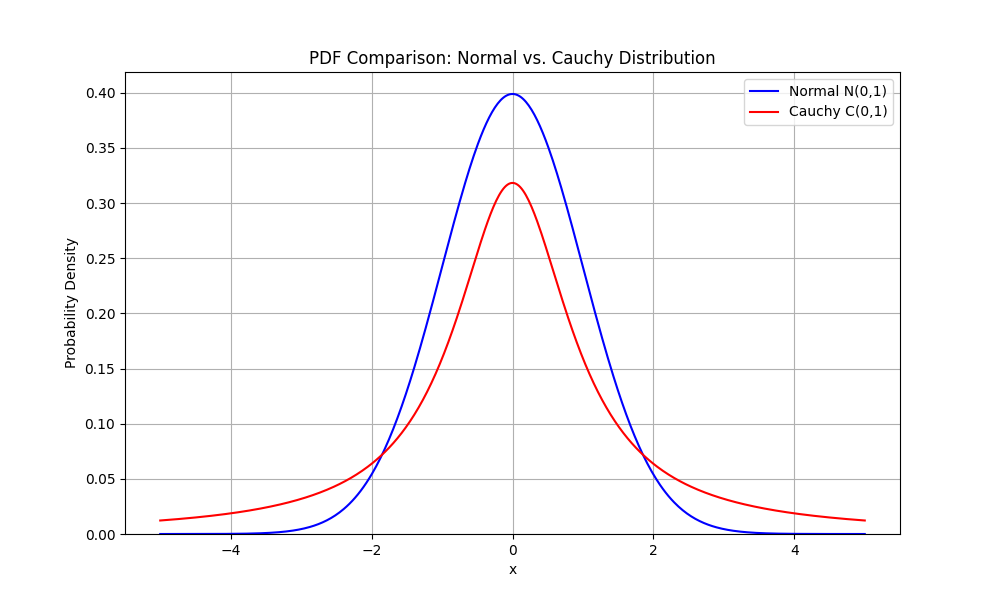
\includegraphics[width=\linewidth]{pdf_normal_cauchy_comparison.png} % Width relative to column
                \caption{PDFs: N(0,1) vs C(0,1)} % Shortened, unnumbered caption
            \end{figure}
            \textbf{对LLN的影响:}
            \begin{itemize}
                \item 不满足LLN的"期望存在/方差有限"条件。
                \item i.i.d. 柯西序列的样本均值\alert{不收敛}。
            \end{itemize}
        \end{column}
    \end{columns}

\end{frame}

% Inserted from gemini_2_5pro.tex
\begin{frame}[shrink=10]{可视化:正态 vs. 柯西样本均值路径}
    \framesubtitle{样本均值随样本量 $n$ 变化的轨迹}
    \begin{columns}[T] % T for top alignment
        \begin{column}{0.5\textwidth}
            \centering
            \textbf{正态分布 $N(0,1)$}\\($\E(X)=0$, $\Var(X)=1$)
            \begin{figure}
                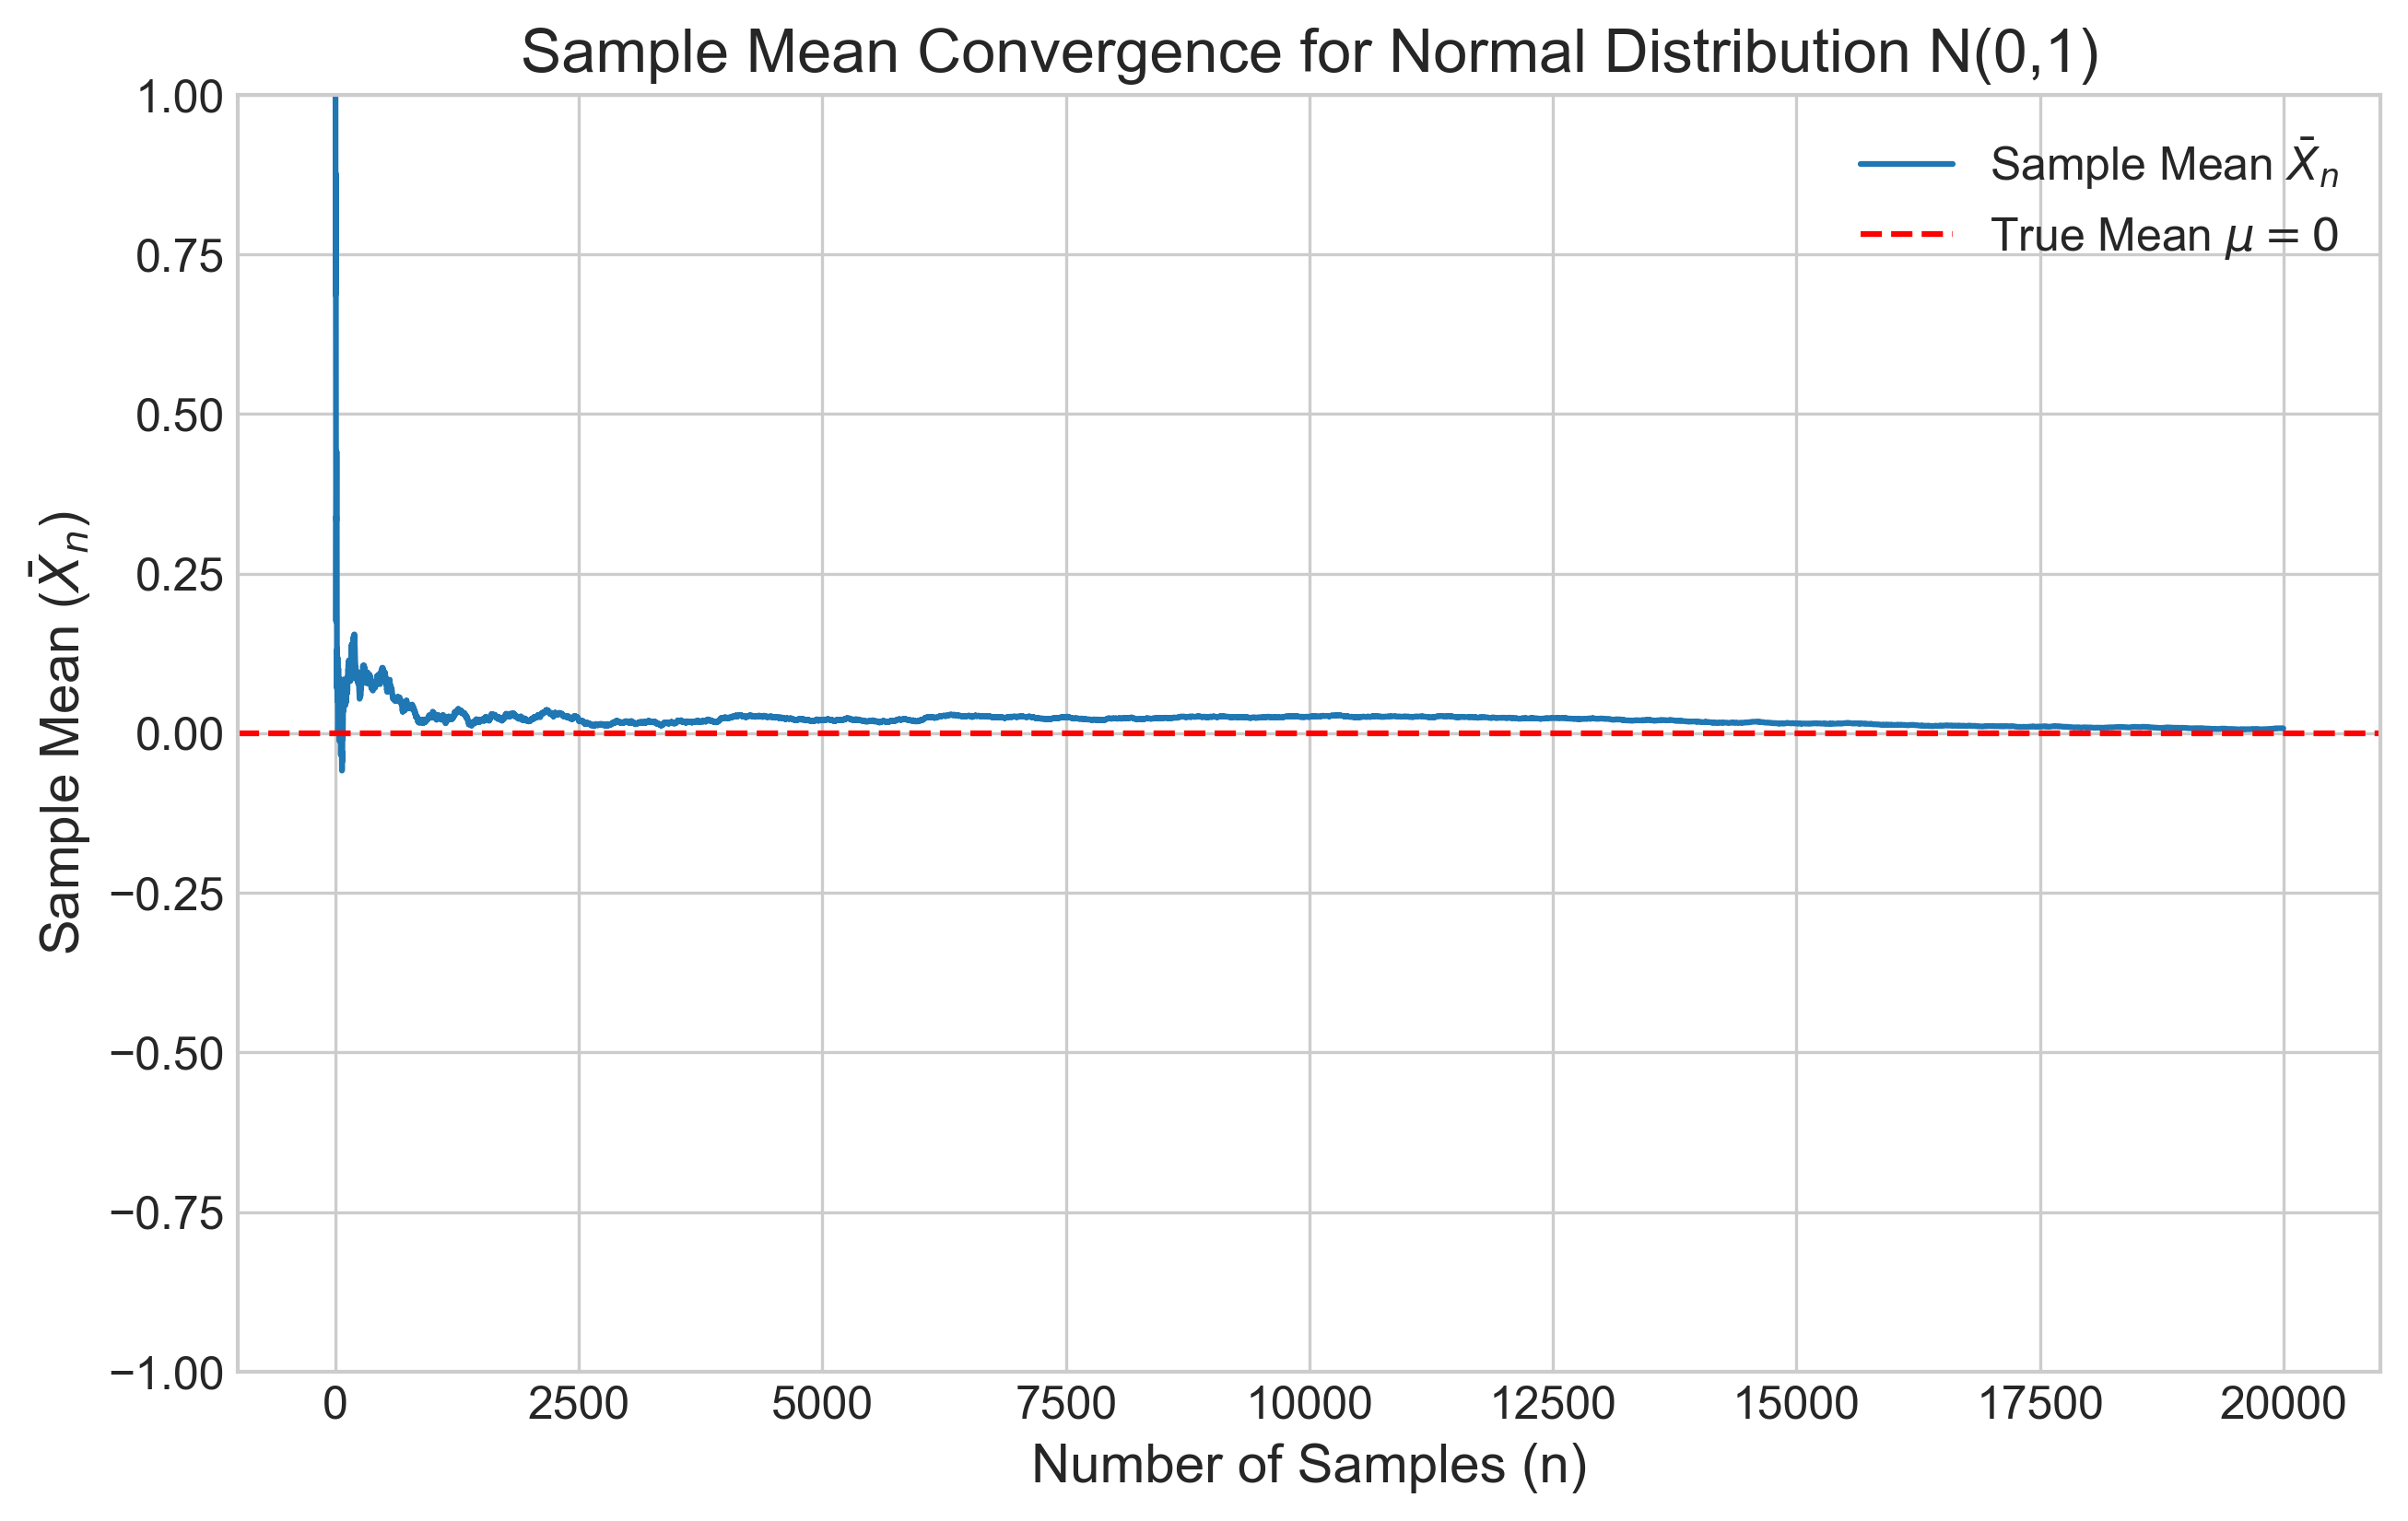
\includegraphics[width=\linewidth]{normal_mean_convergence.png}
                \caption{$\bar{X}_n$ 快速稳定收敛到 $\mu=0$}
            \end{figure}
        \end{column}
        \begin{column}{0.5\textwidth}
            \centering
            \textbf{柯西分布 $C(0,1)$}\\($\E(X)$ 不存在)
            \begin{figure}
                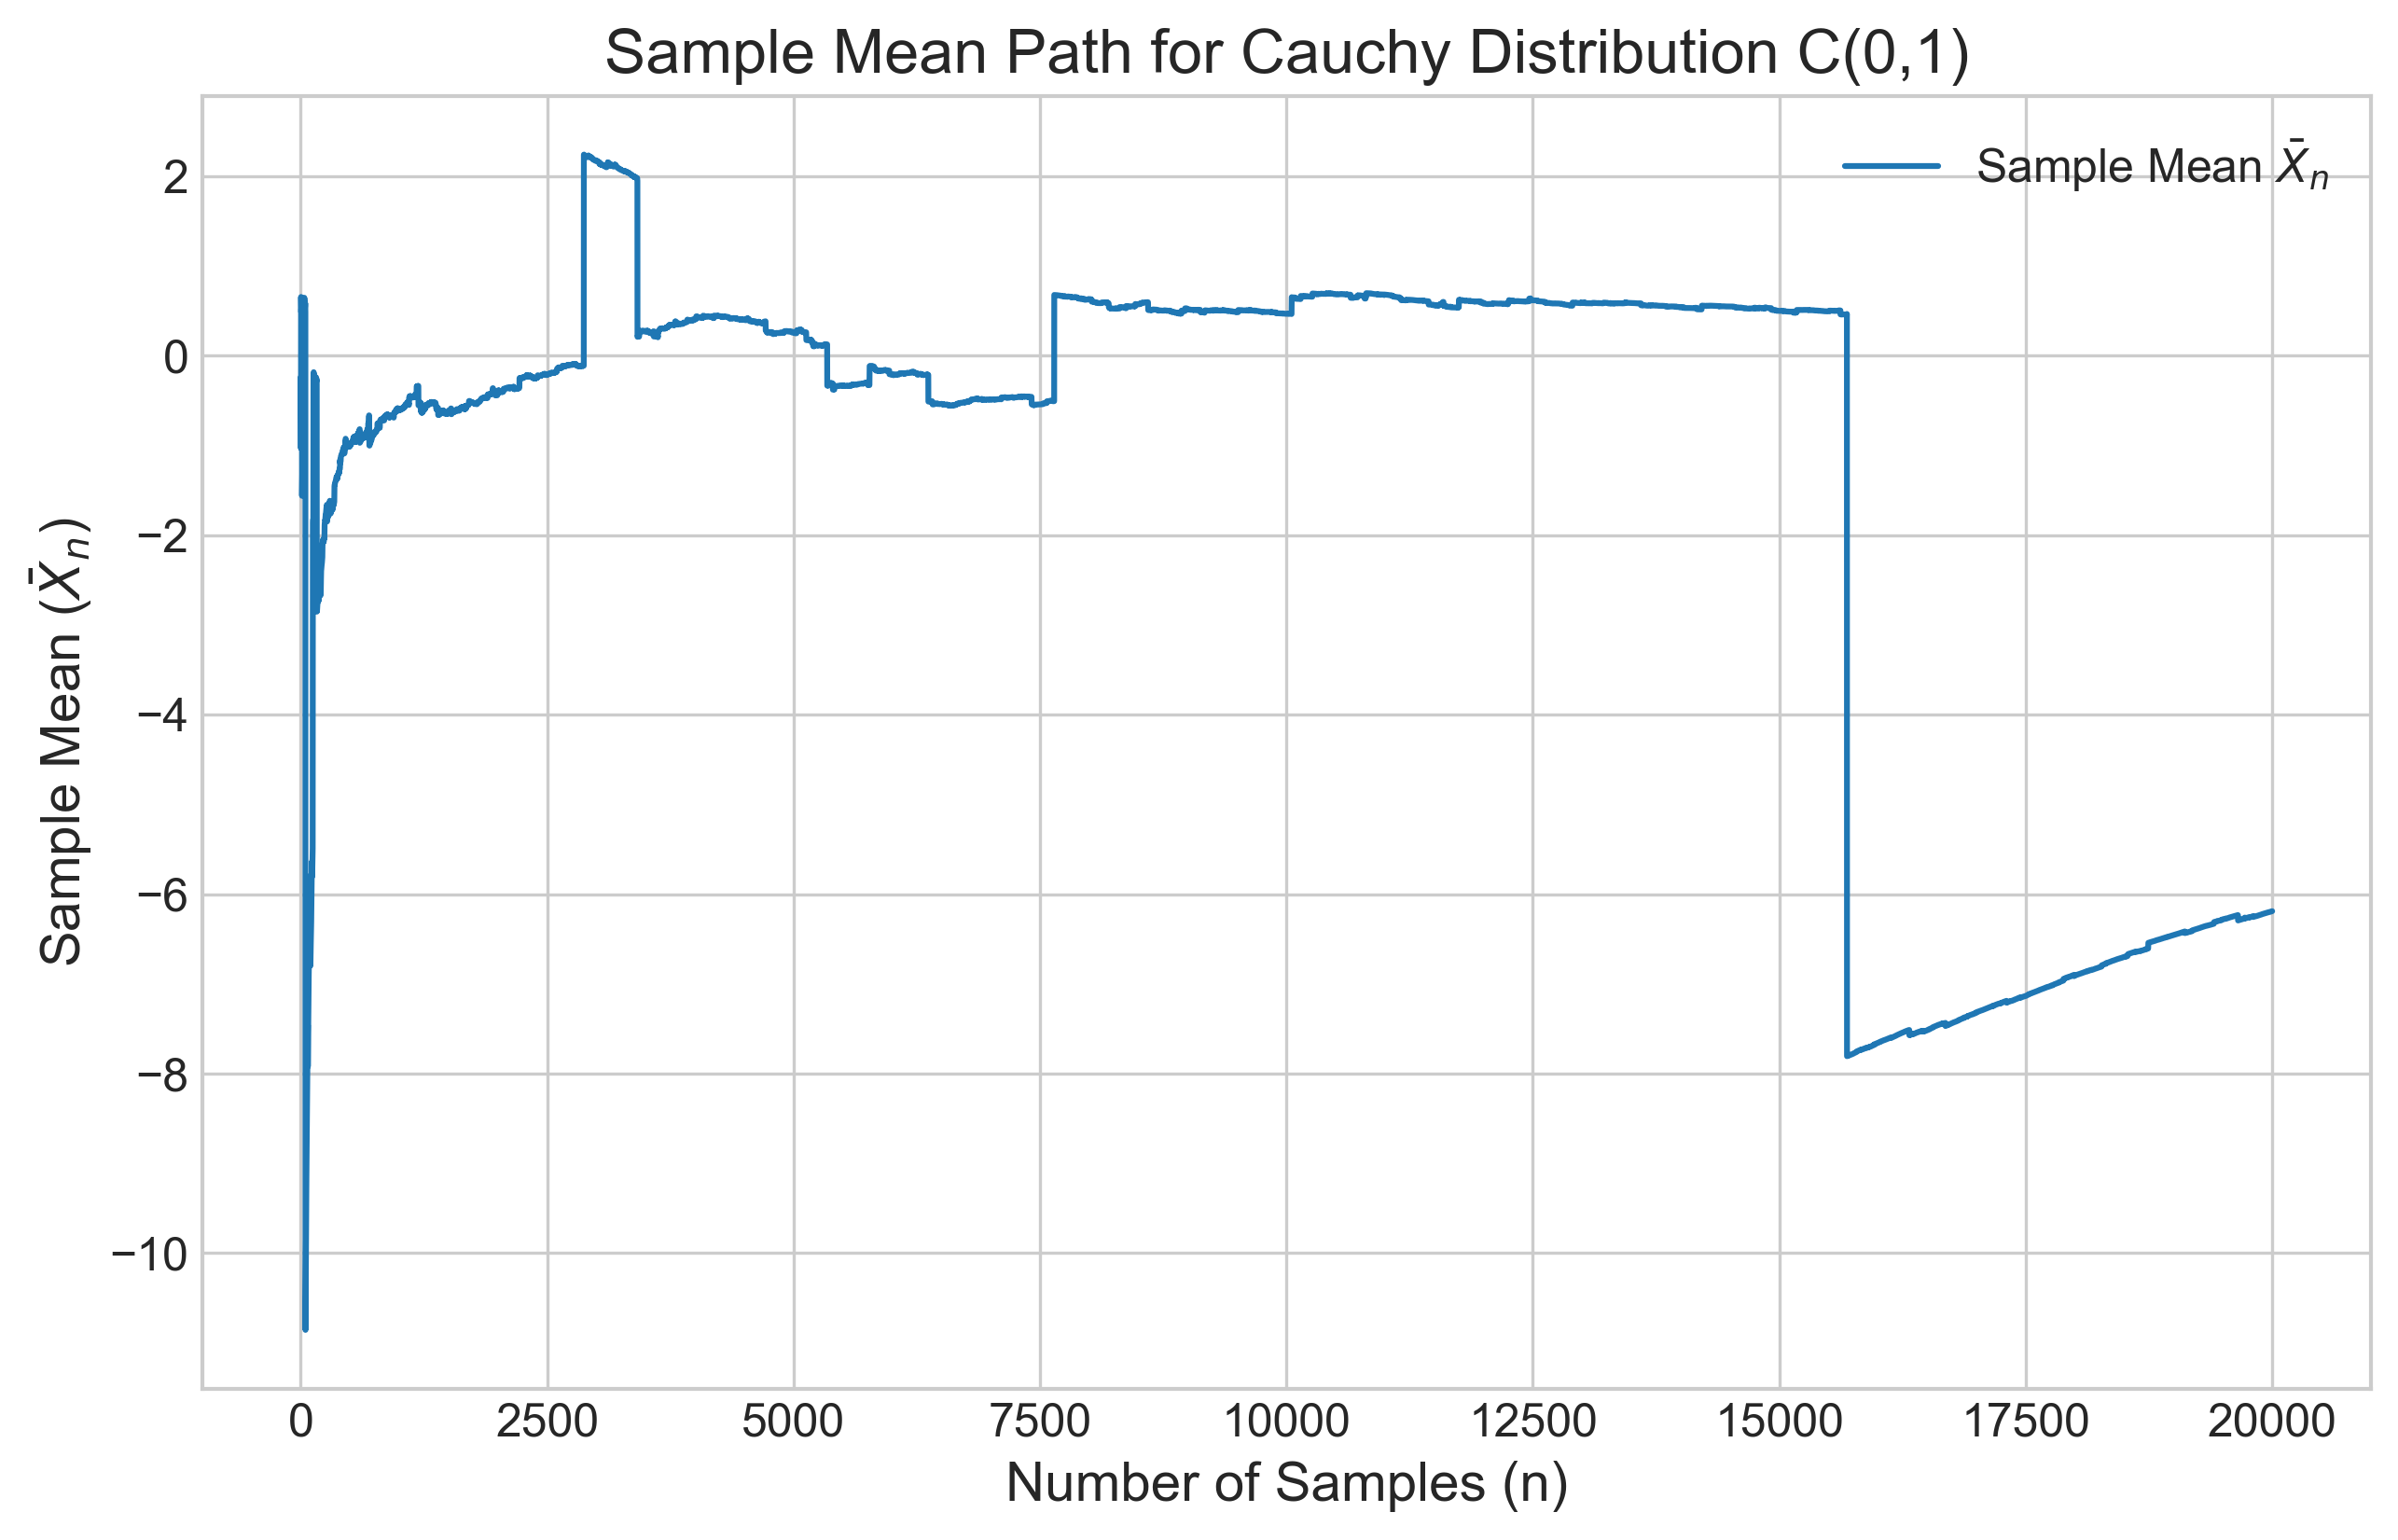
\includegraphics[width=\linewidth]{cauchy_mean_no_convergence.png}
                \caption{$\bar{X}_n$ 持续剧烈波动, \alert{不收敛}}
            \end{figure}
        \end{column}
    \end{columns}
    \vspace{0.2cm}
    \centering
    \textbf{柯西样本均值:持续波动,不收敛 (极端值影响)}
    % \begin{itemize}
    %     \item 正态样本均值:稳定收敛 (符合LLN)。
    %     \item 柯西样本均值:持续波动,不收敛 (极端值影响)。
    % \end{itemize}
\end{frame}
% End of inserted content

% 修改辛钦弱大数定律幻灯片
\begin{frame}[shrink=10]{辛钦弱大数定律 (Khinchin's WLLN)}
    \framesubtitle{期望存在即可保证依概率收敛 (i.i.d.情况)}
    辛钦WLLN:i.i.d.序列,仅要求\alert{期望存在} (无需方差有限)。
    \vspace{0.3cm}
    \begin{block}{定理 7.4 (辛钦弱大数定律)} % Number changed to 7.4
        设 $X_1, X_2, \dots, X_n, \dots$ 是一列\alert{独立同分布 (i.i.d.)} 的随机变量序列,且其共同的期望 $\E(X_i) = \mu$ \alert{存在} (即 $|\mu| < \infty$)。
        令样本均值为 $\bar{X}_n = \frac{1}{n} \sum_{i=1}^{n} X_i$。
        则对于任意 $\epsilon > 0$,有:
        \[ \lim_{n \to \infty} \Prob(|\bar{X}_n - \mu| \geq \epsilon) = 0 \]
        即 $\bar{X}_n \xrightarrow{P} \mu$。
    \end{block}
    \vspace{0.3cm}
    \textbf{柯西分布与辛钦WLLN:}
    \begin{itemize}
        \item i.i.d.柯西序列:期望\alert{不存在} $\implies$ \alert{不满足}辛钦WLLN条件。
        \item 结论:其样本均值 $\bar{X}_n$ \alert{不}依概率收敛。
    \end{itemize}
\end{frame}


\section{强大数定律 (SLLN)}
% 修改强大数定律幻灯片
\begin{frame}[shrink=10]{7.3 强大数定律 (Strong Law of Large Numbers, SLLN)}
    \framesubtitle{样本均值的几乎必然收敛 (更强的收敛)}
    SLLN:更强收敛性,样本均值\alert{几乎必然收敛} ($\xrightarrow{a.s.}$)于总体期望 (同样要求期望存在)。
    \vspace{0.3cm}

    \begin{block}{定理 7.5 (柯尔莫哥洛夫强大数定律)} % Number changed to 7.5
        设 $X_1, X_2, \dots, X_n, \dots$ 是一列\alert{独立同分布 (i.i.d.)} 的随机变量序列,且其共同的期望 $\E(X_i) = \mu$ \alert{存在} (即 $|\mu| < \infty$) 。
        令样本均值为 $\bar{X}_n = \frac{1}{n} \sum_{i=1}^{n} X_i$。则:
        \[ \Prob\left( \lim_{n \to \infty} \bar{X}_n = \mu \right) = 1 \]
        这表示样本均值 $\bar{X}_n$ \alert{几乎处处收敛} (Almost Surely Converge) 于 $\mu$,记作 $\bar{X}_n \xrightarrow{a.s.} \mu$。
    \end{block}
    \vspace{0.3cm}
    \textbf{柯西分布与SLLN:}
    \begin{itemize}
        \item i.i.d.柯西序列:期望\alert{不存在} $\implies$ \alert{不满足}SLLN条件。
        \item 结论:其样本均值 $\bar{X}_n$ \alert{不}几乎必然收敛。
    \end{itemize}
    \footnotesize
    \textit{注:柯尔莫哥洛夫强大数定律的条件与辛钦弱大数定律相同 (i.i.d.且期望存在),但结论更强。}
\end{frame}

% 修改WLLN 与 SLLN 的区别与联系幻灯片:加入正态 vs 柯西对比
\begin{frame}{WLLN 与 SLLN 的区别与联系 (1):正态分布}
    \framesubtitle{依概率收敛 vs. 几乎必然收敛}
    \textbf{核心区别}:
    \begin{itemize}
        \item \textbf{WLLN - \alert{依概率收敛} ($\xrightarrow{P}$)}: $\lim_{n \to \infty} \Prob(|\bar{X}_n - \mu| \geq \epsilon) = 0$. 关注\alert{概率}的极限。
        \item \textbf{SLLN - \alert{几乎必然收敛} ($\xrightarrow{a.s.}$)}: $\Prob(\lim_{n \to \infty} \bar{X}_n = \mu) = 1$. 关注\alert{样本路径}的极限。
    \end{itemize}
    \pause
    \textbf{条件与对比:}
    \begin{itemize}
        \item SLLN 比 WLLN \alert{更强} ($\xrightarrow{a.s.} \implies \xrightarrow{P}$)。
        \item 两者最广泛应用的 i.i.d. 版本都要求 \alert{期望存在} ($|\mu| < \infty$)。
        \item \textbf{对于正态分布 (例如 $N(\mu, \sigma^2)$):}
            \begin{itemize}
                \item 期望 $\mu$ 存在、方差 $\sigma^2$ 有限 $\implies$ 满足LLN条件。
                \item i.i.d. 正态样本均值 $\bar{X}_n$: $\xrightarrow{P} \mu$ 且 $\xrightarrow{a.s.} \mu$。
            \end{itemize}
%        \item \textbf{对于柯西分布:}
%            \begin{itemize}
%                \item 期望\alert{不存在}。不满足大数定律的期望存在条件。
%                \item i.i.d.柯西随机变量的样本均值 $\bar{X}_n$ \alert{不}依概率收敛于任何常数。
%                \item i.i.d.柯西随机变量的样本均值 $\bar{X}_n$ \alert{不}几乎必然收敛于任何常数。
%                \item \alert{惊人事实}:若 $X_1, \dots, X_n$ i.i.d. 服从标准柯西分布,则它们的样本均值 $\bar{X}_n = \frac{1}{n} \sum_{i=1}^n X_i$ \alert{仍服从标准柯西分布}! (与 $n$ 无关)
%            \end{itemize}
    \end{itemize}
\end{frame}

\begin{frame}{WLLN 与 SLLN 的区别与联系 (2):柯西分布反例}
    \framesubtitle{期望不存在导致大数定律失效}
 
    \centering
    \begin{tabular}{lcc}
        \toprule
        \textbf{特性} & \textbf{正态分布} & \textbf{柯西分布} \\
        \midrule
        均值 & 存在 ($\mu$) & 不存在(位置参数 $x_0$) \\
        \midrule
        方差 & 有限 ($\sigma^2$) & 不存在(尺度参数 $\gamma$) \\
        \midrule
        LLN & 成立 & 不成立  \\
        \midrule
        样本均值行为 & 收敛至 $\mu$ & 剧烈波动 \\
        \bottomrule
    \end{tabular}
    \vspace{0.5cm} % Add some space after the table
    \par % New paragraph before the caption-like text
    \centering % Center the caption text
    \small % Make the caption text a bit smaller
    表:正态分布与柯西分布对比

    \pause
    \vspace{0.5cm}
    \leftskip=0.5cm

    \textbf{关键特性:}对于i.i.d.柯西序列的样本均值 $\bar{X}_n$
    \begin{itemize}
       \item 期望\alert{不存在} $\implies$ 不满足LLN的期望存在条件, 即
        \[ \bar{X}_n \not\xrightarrow{P} \text{const}, \quad \bar{X}_n \not\xrightarrow{a.s.} \text{const} \]
       \item \alert{惊人事实}:若 $X_i \sim C(0,1)$ i.i.d., 则 $\bar{X}_n = \frac{1}{n} \sum X_i \sim C(0,1)$ (\alert{仍为标准柯西分布}, 与 $n$ 无关!)
    \end{itemize}
    \vspace{0.3cm}
\end{frame}


\section{大数定律的应用}
% Shrink may be needed
\begin{frame}{7.4 大数定律的应用 (Applications of LLN)}
    \framesubtitle{应用广泛,但基础是满足LLN条件 (尤其期望存在)}
    \begin{itemize}
        \item \textbf{前提}:应用均假设满足LLN条件 (尤其\alert{期望存在})。
        \item \textbf{理论与解释}:
            \begin{itemize}
                \item \alert{频率稳定性} (伯努利LLN)。
                \item 解释平均结果的稳定趋向。
            \end{itemize}
        \item \textbf{统计推断}:
            \begin{itemize}
                \item \alert{参数估计} (样本均值 $\rightarrow$ 总体期望, \alert{前提:期望存在!})。
                \item \alert{蒙特卡洛方法} (随机抽样估计)。
            \end{itemize}
        \item \textbf{风险管理与保险}:预测平均赔付。
        \item \textbf{质量控制}:样本推断总体。
        \item \textbf{物理与工程}:多次测量取平均减小误差。
            \begin{itemize}
                \item \textit{警示:若误差为柯西分布,平均\alert{无效}!} 
            \end{itemize}
    \end{itemize}
    \vspace{0.2cm}
    \alert{核心警示}:LLN条件 (尤其期望存在) 是应用有效的关键。
\end{frame}

\section{总结与展望}
% Shrink may be needed
\begin{frame}{总结与展望}
    \begin{block}{本讲小结}
        \begin{itemize}
            \item \textbf{切比雪夫不等式}: 概率上界 (需方差)。
            \item \textbf{弱大数定律 (WLLN)}: $\bar{X}_n \xrightarrow{P} \mu$ (如辛钦: i.i.d., $\E X_i$存在)。
            \item \textbf{强大数定律 (SLLN)}: $\bar{X}_n \xrightarrow{a.s.} \mu$ (如柯尔莫哥洛夫: i.i.d., $\E X_i$存在); SLLN $\implies$ WLLN.
            \item \alert{LLN条件核心}: \textbf{期望存在性}。
            \item \alert{反例 - 柯西分布}: $\E X$不存在 $\implies$ LLN不适用; $\bar{X}_n$仍为柯西。
            \item \textbf{LLN地位}: 连接概率论与统计实践的\alert{核心桥梁}。
        \end{itemize}
    \end{block}
\end{frame}

\begin{frame}
    \begin{alertblock}{展望}
        \begin{itemize}
            \item 大数定律描述了\alert{平均}行为的极限。
            \item 核心极限定理 \alert{中心极限定理 (CLT)}:描述样本均值的\alert{分布} $\rightarrow$ 正态分布 (通常需 $\E X, \Var X$ 存在)。
            \item 大数定律和中心极限定理共同构成了现代统计推断的理论基石。
        \end{itemize}
    \end{alertblock}
\end{frame}

\begin{frame}
    \centering
    \Huge{\bfseries 谢谢聆听!}
    
    \vspace{0.5cm} % Adjusted spacing a bit
    \normalsize
    相关数学证明参考资料请访问: \\
    \texttt{https://1587causalai.github.io/BasicProbabilityLectureNotes}

    \vspace{1cm}
    \normalsize
    问题与讨论
\end{frame}

\end{document}